\documentclass[useAMS,usenatbib]{mn2e}
%%%%% AUTHORS - PLACE YOUR OWN MACROS HERE %%%%%%%%%%%%%%%%%%
\usepackage{graphicx}
\usepackage{epstopdf}
\epstopdfsetup{outdir=./}
\usepackage{color}
%\usepackage{floatpag}
\usepackage[pdftex, hidelinks]{hyperref}
\newcommand {\aplt} {\ {\raise-.5ex\hbox{$\buildrel<\over\sim$}}\ }
%\setlength\parindent{0pt}
%%%%%%%%%%%%%%%%%%%%%%%%%%%%%%%%%%%%%%%%%%%%%%%%


\title[The SGP at 145\,MHz with PAPER]{Measurements of the Southern Galactic Plane at 145\,MHz with PAPER}

\author[S. A. Kohn et al.]{S.~A. Kohn,$^{1}$\thanks{E-mail: saulkohn@sas.upenn.edu} J.~E. Aguirre,$^{1}$ W.~R. Saunders,$^{1}$
A.~R. Parsons,$^{2,3}$
\newauthor et al.$^4$\\
$^{1}$ Department of Physics and Astronomy, University of Pennsylvania, Philadelphia, PA 19104\\
$^{2}$ Astronomy Dept., U. California, Berkeley CA\\
$^{3}$ Radio Astronomy Lab., U. California, Berkeley CA\\
$^{4}$ a lot of other places\\
}
\begin{document}
\date{}

\pubyear{2015}
\maketitle
\begin{abstract}
Present astrophysical understanding of high-mass stars allows for predictions of their formation rates.  High-mass stars explode in supernovae, which leave behind Supernova Remnants (SNRs) that serve as records of the stars; however the $\sim$300 observed SNRs is far fewer than the $>1000$ predicted.  This ``SNR Defect" could implicate the understanding of high-mass stars if confirmed. 
Meanwhile, there is presently a dearth of low-frequency radio measurements ($\nu\aplt$200\,MHz) of sources in the Southern Galactic Plane (SGP).
This study reports on a search for SNRs as well as measurements of other sources in the SGP using low-frequency radio maps produced at 145\,MHz by Precision Array for Probing the Epoch of Reionization (PAPER).
For several known SNR positions we do not detect significant flux above background, suggesting a synchrotron self-absorption mechanism at play for these particular SNRs. The implications of our SNR detection rate is discussed with a focus on the SNR Defect. We also detect several H{\sc ii} regions, which are unexpected at these low frequencies due to the sharp spectral fall-off of free-free emission. 
\end{abstract}

\begin{keywords}
ISM: molecular clouds -- stars: formation
\end{keywords}

\section{Introduction}
\label{sec:intro}
The Southern Galactic Plane (SGP) has been measured at various radio frequencies, including the Molonglo Galactic Plane Surveys \citep[MGPS-1 and 2;][]{Green.99,Murphy.07} and the Molonglo Observatory Synthesis Telescope SNR Catalog \citep[MOSTSNRCAT;][]{Whiteoak.96} at 843\,MHz and the Southern Galactic Plane Survey \citep[SGPS;][]{Haverkorn.06} at 1.4\,GHz. Synthetic catalogs of SNRs at 1\,GHz \citep[][hereafter G14]{DAGreen.14} and H{\sc ii} regions at 2.7\,GHz \citep[][hereafter P03]{Paladini.03} also cover the SGP, and infrared measurements were made by, e.g., the Midcourse Space Experiment \citep[MSX;][operating at 8.28--21.3\,$\mu$m (36.23--14.08\,THz)]{Egan.03}. 

However, there is a dearth of measurements of the SGP at low radio frequencies ($\nu\aplt$200\,MHz). In this work, we present measurements of the SGP at a central frequency of 145\,MHz as measured by the Precision Array for Probing the Epoch of Reionization (PAPER\footnote{\url{eor.berkeley.edu}}). Currently the only counterparts to such measurements were presented in the 7C(G) survey of the Northern Galactic Plane \citep{Vessey.98} which was conducted at 151\,MHz, and the GaLactic Extragalactic All-sky MWA\footnote{\url{www.mwatelescope.org}} (GLEAM) survey, which is currently processing its data in five 30\,MHz bands centered at 88, 118, 154, 185 and 216\,MHz \citep{Wayth.15}.

\subsection{Supernova Remnants}
The major classification difference between high-mass ($M > 8M_{\odot}$ ) and low-mass ($M < 8 M_\odot$) stars is the end of their life, for which the latter explode in supernovae (SNe), which is precipitated by accumulated inert iron in the core \citep{Arnett.73}.  
The subsequent collapse of the core creates the supernova explosion, which ejects the entirety of the star’s outer layers, forming a supernova remnant (SNR).  The SNR consists of the expanding supernova shock wave, the ejected outer material of the star, and any dust or gas it picks up while expanding.  
The remnant slowly expands until its density becomes near that of the surrounding interstellar medium (ISM) making it effectively indistinguishable, and ending its existence as an SNR.  

The SNR shock releases high-velocity particles, including a barrage of electrons that produce non-thermal emissions; these relativistic electrons are accelerated and spiraled by the magnetic fields of the SNR and produce synchrotron radiation as a result making SNRs easily-detectable radio sources \citep[e.g.][]{Burbidge.56,Stupar_cat.11}. 
SNRs are relatively short-lived ($\sim10^5$ yr), which means that they can serve as a record of recent star formation rates of high-mass stars -- by counting SNRs, one can hope chart recent star formation.
Measuring the star formation rates through iron abundance allows for a reasonable prediction of the number of galactic SNRs; however, these predictions imply that there should be far more SNRs than currently detected \citep[e.g.][]{Brogan.06}.  

To date, 294 SNRs have been catalogued G14 despite the prediction based on the Galactic star formation rate that $\sim10^3$ galactic SNRs exist \citep{Li.91,Pavlovic.13}.  
Additionally, \cite{Brogan.06} made estimates based on known limitations of radio surveys in order to predict the number of SNRs that are observable at all.
Their study yielded a result of 460 observable SNRs; this is still less than half of the observed value. 
This “SNR Defect” has thus far been attributed to selection effects including: 
\begin{itemize}
\item SNRs occur in dusty regions, where the dust may absorb and/or deflect SNR emissions;
\item since the vast majority of stars are located along the galactic plane, so are most SNRs, increasing potential source confusion \citep[e.g.][]{Gao_v.11,Gao_vi.11};
\item due to the inverse square law of observed luminosity,% doubling the distance to an object reduces its apparent brightness by one-fourth. 
the light from SNRs located 50,000 ly away, for example, is diminished by a factor of $\sim$300  \citep{Green.91};
\item superpositioning along the Earth’s line of sight, by which nearby, young  and inherently dense SNRs block or severely inhibit the entire field of view behind them, making surveys of the SNR population more difficult. 
\end{itemize}

Radio observations should be able to resolve some of these selection effects. Dust neither attenuates nor scatters at radio frequencies. Young SNRs, which are compact and have close-to-blackbody emission spectra are more easily detected by optical surveys, whereas older SNRs, which are more diffuse and emit mostly at lower frequencies, are better detected with radio surveys.

\subsection{H{\sc ii} regions and misidentification}
While observing at radio frequencies mitigates most of the confusion when observing the Galactic plane, H{\sc ii} regions pose a more significant problem.  H{\sc ii} regions, opposed to SNRs, thermally emit from heating caused by nearby OB stars.
For example, SNR G166.2+2.5 was discovered to be an H{\sc ii} region heated by O7.5V star BD+41 1144 \citep{Foster.06}.  

Some larger SNRs, such as W28 (18h01m22.7s -23$^{\circ}$17'20") and W30 (18h03m -21$^{\circ}$30'), have positioned within them H{\sc ii} regions and other sources of thermal emissions, which increase the likelihood of misidentification \citep{Andrews.85}. \cite{Brogan.06} showed that the small likelihood of actual proximity notwithstanding, the apparent proximity interferes with detection of SNRs.  As a result, much has been invested in finding a method to mitigate the selection effects.\\

This work presents measurements of sources in the SGP using PAPER, a low-frequency radio telescope that observes at a central frequency of 145\,MHz. The paper is laid out as follows. In section~\ref{sec:obs} we discuss the acquisition and reduction of PAPER's measurements of the SGP. Section~\ref{sec:res} presents our map of the SGP, with detections of SNRs, H{\sc ii} regions and extragalactic sources cross-matched with the many of the catalogs listed above. We also investigate those sources which do not match with any of the catalogs. In Section~\ref{sec:disc} we discuss our findings, with a focus on the SNR Defect. We summarize and conclude our study in Section~\ref{sec:conc}.

\section{Observations and data reduction}
\label{sec:obs}

The Precision Array for Probing the Epoch of Reionization (PAPER) is an experiment designed to set the strongest limits on, and possibly detect, the 21\,cm signal of neutral hydrogen at redshifts $z \geq 7.5$. It is operated in the Karoo, South Africa (-30:43:17.5 N, 21:25:41.9 E). To be able to set the strong limits it has to date \citep{Parsons.14, Jacobs.14, Ali.15, Moore.15}, it requires a highly redundant configuration to maximise its sensitivity to a few discrete uvw voxels \citep{Parsons.12}. However, in July and September 2011 the array was briefly reconfigured into an imaging (i.e. maximally non-redundant) array in order to do image-based analysis of the low-frequency radio sky \citep[e.g.][]{Jacobs.11, Stefan.13}. The imaging configuration and its instantaneous uv coverage is shown in Figure~\ref{fig:config}. Antennae were arranged in a pseudo-random scatter within a 300\,m-diameter circle, granting resolutions between 15' and 25' across the band.
Drift-scan visibilities were measured every 10.7 s, and divided into datasets about 10 minutes in length. PAPER antennae cannot point. However, within each dataset we are able to phase to the median zenith post-data-acquisition, and image accordingly. In this work we present single-polarization measurements made overnight July 4--5th 2011.

All calibration was performed using the Astronomical Interferometry in PYthon ({\sc{aipy}}) package\footnote{\url{https://github.com/AaronParsons/aipy}}.
Cross-talk removal was performed, and RFI removal masked channels that persistently showed large deviations from smooth-spectrum foregrounds (mainly due to known communications satellite bands). This removed approximately 30\% of the available bandwidth, and most removal occurred at the high and low ends of the band -- PAPER's excellent RFI environment allows most of the contiguous band to be used. Visibilities of bright extragalactic radio sources (e.g. Virgo A, Cygnus A) were modelled and removed from the data. 

XXX FROM FOLIO ARCHAEOLOGY -- WOULD LIKE CONFIRMATION FROM AARON XXX
Absolute calibration was achieved by phasing to Pictor A, and adjusting the overall gain and phase of the array accordingly \citep{Jacobs.13}.

The data sets were self-calibrated to obtain complex gain solutions for each antenna, and then imaged, averaging over the whole 100\,MHz-wide band. Each image (dataset) was w-projected with a uv matrix resolution of 0.4 and a w-plane resolution of 0.1, and CLEANed \citep{Clark.80} to one part in $10^4$. These images were then used as `facets' and gridded to a HEALPix \citep{Gorski.05, Gorski.11} sphere with pixel size of 1 arcmin, subsequently convolved with a 2D Gaussian (FWHM=6 arcmins) to reduce pixelization effects. Finally, a cut in Galactic coordinates was made to extract the SGP ($25<l<230$, $-7.5<b<7.5$).

\begin{figure}
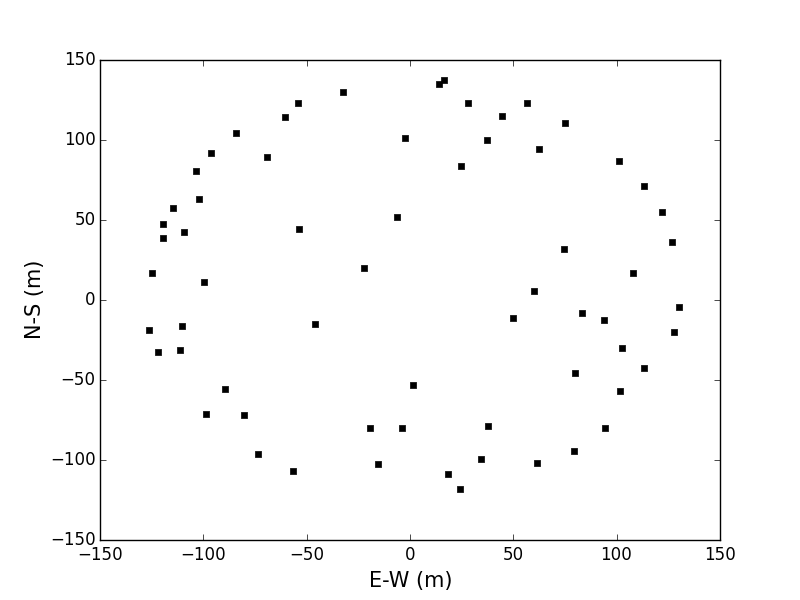
\includegraphics[width=\columnwidth]{figs/psa64imageconfig.png}
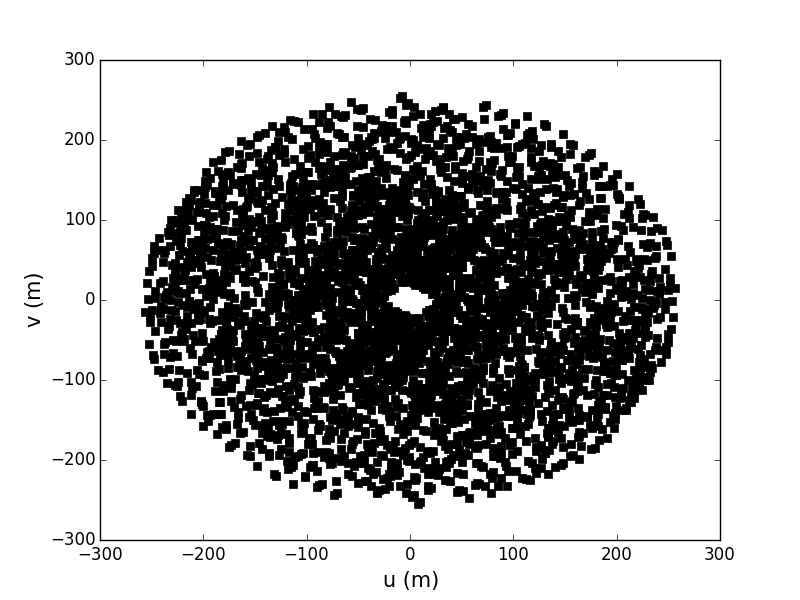
\includegraphics[width=\columnwidth]{figs/psa64uvcoverage.png}
\caption{\textit{Above}: The PAPER-64 single-polarization configuration that took the measurements we report on in this paper. The antennae were arranged in a pseudo-random scatter in order to optimize uv-coverage. \textit{Below}: The resultant instantaneous uv-coverage, masking the very-short baselines ($\aplt 10 \lambda$). Maximum voxel occupancy is $\sim10$.}
\label{fig:config}
\end{figure}

\section{Results}
\label{sec:res}

Our map of the SGP is shown in Figure~{\color{red}[NUMBER]}. Contours are at XXX, XXX... Jy\,beam$^{-1}$. 

Source identification and extraction was performed using PyBDSM\footnote{\url{http://www.lofar.org/wiki/doku.php?id=public:user software:pybdsm}}, which identified all sources $\geq5\sigma$ above their local background, accounting for possible sidelobe confusion \citep{PyBDSM.15}. The average background noise is $\sim$1\,Jy, so our detection threshold is $\sim$5\,Jy. To each detected source we XXX fit (not the right word) XXX a two-dimensional, 20' FWHM Gaussian to approximate the PAPER beam \citep{Parsons.10} in order to extract the integrated source flux, size, and uncertainties on these. 

We detected 230 individual sources, 120 of which were resolved to sufficient quality that we can report their flux with confidence, XXX and 21 of which were flagged as ``uncertain" but worth reporting XXX. The remaining 89 were too confused; largely in the most crowded areas of the SGP ({\bf COORDS, FIG NUM \& LETTER}). In order to identify each source, we checked if any known sources were within the 20' PAPER beam at that position in the Galactic radio catalogues described in the introduction: MGPS, MOSTSNRCAT, the \cite{AGreen.14} and G14 SNR catalogues and the P03 H{\sc ii} region catalogue. We also matched to the extragalactic Molongolo Reference Catalogue \citep[MRC;][]{Large.81} sources detected in \cite{Jacobs.11}, a few of which (28) overlapped with our SGP cut. 

XXX In the case of double-matches... XXX

For the detected sources that were not within 20' of any objects in these catalogues (23), we queried the SIMBAD astronomical database \citep{Wegner.00} for any other SNRs,  IR bubbles, H{\sc ii} regions or undetected radio sources within the semi-major axis of the source.

PAPER is not able to reconstruct flux on scales greater than $\sim3$ degrees due to missing baselines.  There is also the problem of source confusion -- due to PAPER's low resolution, we can only be confident of our measurements if a source isolated.

\subsection{Comparison of SNR catalogues with PAPER measurements}
\label{subsec:G14}

We cross-matched our detections with SNR catalogues MOSTSNRCAT, \cite{AGreen.14} and G14. There is a large degree of degeneracy between the MOSTSNRCAT and G14 catalogues. We only detect one MOSTSNRCAT source not listed in the G14 catalogue (G315.4-2.3), but in a confused region -- it is not isolated enough to reliably calculate a flux density for. 

\cite{AGreen.14} find 23 new SNRs identified in MGPS (843\,MHz) that are not in the G14 catalogue. Of these 23 we detect 7 (which is expected given the relatively low fluxes of many of the SNRs found in their survey, requiring unrealistically large spectral indices to be detectable by PAPER), and of the 7 we detect there are 3 that are isolated enough to perform analyses. Their properties are listed in Table~\ref{tab:AG}, where we show the SNRs' identifier, coordinates, and the size of the semi-major axis (SMA) as measured by \citep{AGreen.14}, along side our measurement of the SMA and flux density.

\begin{table*}
\caption{Isolated SNRs detected by \protect\citep{AGreen.14} in MGPS compared with our own measurements}
\begin{tabular}{lllcccc}
\hline
SNR & R.A. & Dec & SMA$^a$ & $S_{843\,{\rm MHz}}$ & SMA (This work) & $S_{145\,{\rm MHz}}$ \\
(G$l\,b$)	&	(deg)	&	(deg)	&	(arcmin)	&	(Jy)		&	(arcmin)			&	(Jy)			\\
\hline
G296.6-0.4 & 178.96 & -62.57 & 14 & $>$0.31 & 22 $\pm$ 1 & 29 $\pm$ 3 \\
G296.7-0.9 & 178.88 & -63.12 & 14 & 2.9 & 17$\pm$3 & 5 $\pm$ 3 \\
G325.0-0.3 & 234.83 & -55.82 & 6   & 0.69 & 42 $\pm$ 6 & 29 $\pm$ 2 \\
\hline
\end{tabular}
\\
$^a$ Green et al. 2014
\label{tab:AG}
\end{table*}

We detect 79 SNRs out of the 294 listed in G14. Of these, 26 are compact, isolated and have well-determined previous radio continuum measurements. Ten are compact and isolated but do not have well-determined previous radio continuum measurements. The remaining 43 are too confused with other sources in the SGP to confidently report their individual fluxes. Higher-resolution low-frequency surveys such as GLEAM, mentioned in Section~\ref{sec:intro}, are required to constrain the nature of SNRs in these crowded regions of the SGP. Meanwhile, there are a further 31 SNRs in the G14 catalogue that are compact, have well-determined previous radio continuum measurements, and have an extrapolated flux $\geq$5\, Jy -- sources that PAPER should detect -- that we do not see. For these sources, synchrotron self-absorption is likely decreasing the low-frequency radio emission.

Here we discuss the different selections of the G14 SNRs mentioned above. We discuss what our numbers mean in terms of the SNR Defect in Section~\ref{sec:disc}.

\subsubsection{SNRs with well-constrained properties}

Twenty six G14 sources are relatively compact and isolated in our SGP map, and have well-determined previous radio continuum measurements. These SNRs are listed in Table~\ref{tab:G14comparison}. For almost all of these sources, our measurements represent the first reported fluxes and sizes at frequencies $<300\,{\rm MHz}$ (the only exception being G008.7-00.1, which was measured at 57.5\,MHz by \citealt{Odegard.86}).

\begin{table*}
\caption{Compact and isolated SNRs from G14 compared with our own measurements.}
\begin{tabular}{llllccccc}
\hline
SNR	&	Other	&	R.A.	&	Dec	&	SMA (G14)	&	$S_{1\,{\rm GHz}}$ &	$\alpha$ 	&	SMA  (This work)			&	$S_{145\,{\rm MHz}}$			\\
(G$l\,b$)	&	Names	&	(deg)	&	(deg)	&	(arcmin)	&	(Jy)	&		&	(arcmin)			&	(Jy)			\\
\hline																					
G004.5+06.8	&	SN1604	&	262.67	&	-21.48	&	3	&	19	&	0.64	&	16.1	$\pm$	0.7	&	16	$\pm$	3	\\
G005.5+00.3	&		&	269.26	&	-24	&	15	&	5.5	&	0.7	&	29	$\pm$	6	&	12	$\pm$	3	\\
G007.7-03.7	&	1814-24	&	274.35	&	-24.06	&	22	&	11	&	0.32	&	18	$\pm$	3	&	8	$\pm$	3	\\
G008.7-00.1	&	W30	&	271.37	&	-21.43	&	45	&	80	&	0.5	&	36	$\pm$	3	&	54	$\pm$	2	\\
G011.2-00.3	&		&	272.86	&	-19.41	&	4	&	22	&	0.5	&	22	$\pm$	2	&	13	$\pm$	3	\\
G018.1-00.1	&		&	276.14	&	-13.18	&	8	&	4.6	&	0.5	&	20	$\pm$	4	&	7	$\pm$	3	\\
G018.8+00.3	&	Kes 67	&	275.99	&	-12.38	&	17	&	33	&	0.46	&	20	$\pm$	1	&	21	$\pm$	3	\\
G018.9-01.1	&		&	277.45	&	-12.96	&	33	&	37	&	0.39	&	28	$\pm$	4	&	22	$\pm$	2	\\
G021.8-00.6	&	Kes 69	&	278.18	&	-10.13	&	20	&	65	&	0.56	&	18.3	$\pm$	0.9	&	23	$\pm$	3	\\
G023.3-00.3	&	W41	&	278.68	&	-8.8	&	27	&	70	&	0.5	&	23	$\pm$	3	&	14	$\pm$	3	\\
G292.0+01.8	&		&	171.15	&	-59.26	&	12	&	15	&	0.4	&	17.9	$\pm$	0.9	&	24	$\pm$	3	\\
G296.7-00.9	&		&	178.87	&	-63.13	&	15	&	3	&	0.5	&	18	$\pm$	3	&	5	$\pm$	3	\\
G296.8-00.3	&	1156-62	&	179.62	&	-62.58	&	20	&	9	&	0.6	&	22	$\pm$	1	&	29	$\pm$	3	\\
G304.6+00.1	&	Kes 17	&	196.49	&	-62.7	&	8	&	14	&	0.5	&	20.7	$\pm$	0.9	&	33	$\pm$	3	\\
G309.8+00.0	&		&	207.62	&	-62.08	&	25	&	17	&	0.5	&	23	$\pm$	1	&	38	$\pm$	3	\\
G315.4-00.3	&		&	218.97	&	-60.6	&	24	&	8	&	0.4	&	27	$\pm$	3	&	22	$\pm$	3	\\
G326.3-01.8	&	MSH 15-56	&	238.25	&	-56.16	&	38	&	145	&	0	&	25.3	$\pm$	0.7	&	125	$\pm$	6	\\
G337.3+01.0	&	Kes 40	&	248.16	&	-46.6	&	15	&	16	&	0.55	&	15.4	$\pm$	0.7	&	16	$\pm$	3	\\
G340.4+00.4	&		&	251.62	&	-44.65	&	10	&	5	&	0.4	&	18	$\pm$	2	&	11	$\pm$	3	\\
G343.1-00.7	&		&	255.1	&	-43.23	&	27	&	7.8	&	0.55	&	23	$\pm$	3	&	15	$\pm$	3	\\
G349.7+00.2	&		&	259.49	&	-37.43	&	2.5	&	20	&	0.5	&	14.8	$\pm$	0.8	&	11	$\pm$	3	\\
G350.0-02.0	&		&	261.95	&	-38.53	&	45	&	26	&	0.4	&	42	$\pm$	7	&	32	$\pm$	2	\\
G352.7-00.1	&		&	261.91	&	-35.11	&	8	&	4	&	0.6	&	20	$\pm$	4	&	8	$\pm$	3	\\
G355.9-02.5	&		&	266.47	&	-33.71	&	13	&	8	&	0.5	&	19	$\pm$	2	&	12	$\pm$	3	\\
G356.2+04.5	&		&	259.75	&	-29.66	&	25	&	4	&	0.7	&	22	$\pm$	4	&	9	$\pm$	3	\\
G357.7-00.1	&	MSH 17-39	&	265.12	&	-30.96	&	8	&	37	&	0.4	&	12.9	$\pm$	0.3	&	22	$\pm$	3	\\
\hline
\end{tabular}
\\
\label{tab:G14comparison}
\end{table*}

The left panel of Figure~\ref{fig:comparisonscatterSNR} shows, for the SNRs in Table~\ref{tab:G14comparison}, the expected 145\,MHz flux calculated by extrapolating the G14 1\,GHz flux by the spectral index reported by that study, highlighting in green those SNRs that G14 report to be compact enough that PAPER should reconstruct all the flux of the SNR. Most of the points lie close to a 1:1 relation (shown in black). However, there appears to be either significant amounts of flux missing i.e. we expect to measure higher fluxes than we actually do. 

XXX INTERPRETATION??? XXX

\begin{figure}
\centering
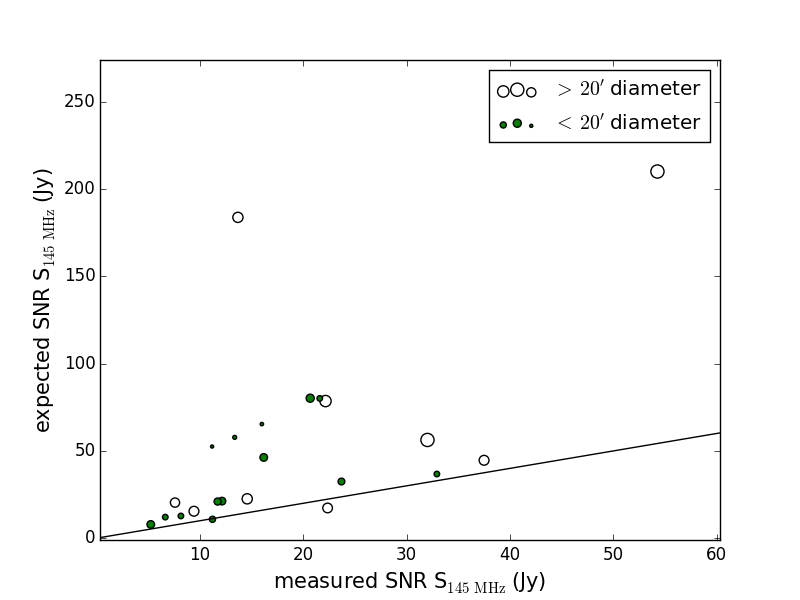
\includegraphics[width=\columnwidth]{figs/GreenScatter.png}
\caption{The fluxes of compact and isolated SNRs (Maj $<$ 3 degrees; PAPER does not have sufficient resolution to detect larger ones) that we measure compared to those expected at 145\,MHz given the G14 1\,GHz fluxes and spectral indices. We highlight in green those SNRs which are compact enough to be completely resolved by the PAPER beam (Maj $<$ 20 arcmin). The size of the point is illustrative of the diameter of the region (as reported by G14, not PAPER), and a black line showing a 1:1 relation is overlaid.}
\label{fig:comparisonscatterSNR}
\end{figure}

\subsubsection{SNRs with uncertain properties}

We detect 10 other SNRs that are isolated and compact in our SGP map, but G14 list as having uncertain radio continuum detection. These sources are often elongated and/or incomplete arcs and shells, or have complex geometries, and are therefore difficult to determine a definite integrated flux for. However, PAPER's resolution is much lower than that of any of the previous studies of these objects. Therefore, the 145\,MHz flux densities of those objects listed in Table~\ref{tab:G14uncertain} may be considered the first fully integrated flux measurements of these SNRs and the regions around them. None of these objects have been observed at frequencies lower than 400\, MHz.

\begin{table*}
\caption{Compact and isolated SNRs that G14 flag as having uncertain radio continuum detections.$^a$}
\begin{tabular}{llllccccc}
\hline
SNR	&	Other	&	R.A.	&	Dec	&	SMA(G14)	&	$S_{1\,{\rm GHz}}$ &	$\alpha$ 	&	SMA(This work)			&	$S_{145\,{\rm MHz}}$			\\
(G$l\,b$)	&	Names	&	(deg)	&	(deg)	&	(arcmin)	&	(Jy)	&		&	(arcmin)			&	(Jy)			\\
\hline			
G013.5+00.2	&		&	273.55	&	-17.2	&	5	&	3.5	&	1.0	&	28	$\pm$	5	&	15	$\pm$	3	\\
G284.3-01.8	&	MSH 10-53	&	154.56	&	-59	&	24	&	11	&	0.3	&	30	$\pm$	2	&	36	$\pm$	3	\\
G289.7-00.3	&		&	165.31	&	-60.3	&	18	&	6.2	&	0.2	&	21	$\pm$	3	&	13	$\pm$	3	\\
G302.3+00.7	&		&	191.47	&	-62.13	&	17	&	5	&	0.4	&	21	$\pm$	2	&	15	$\pm$	3	\\
G312.5-03.0	&		&	215.25	&	-64.2	&	20	&	3.5	&	?	&	25	$\pm$	4	&	15	$\pm$	3	\\
G318.9+00.4$^b$	&		&	224.62	&	-58.48	&	30	&	4	&	0.2	&	21	$\pm$	3	&	11	$\pm$	3	\\
G327.1-01.1	&		&	238.6	&	-55.15	&	18	&	7	&	?	&	18	$\pm$	3	&	6	$\pm$	3	\\
G327.4+00.4	&	Kes 27	&	237.08	&	-53.81	&	21	&	30	&	0.6	&	19	$\pm$	1	&	37	$\pm$	3	\\
G330.2+01.0	&		&	240.27	&	-51.56	&	11	&	5	&	0.3	&	20	$\pm$	2	&	16	$\pm$	3	\\
G351.2+00.1	&		&	260.61	&	-36.18	&	7	&	5	&	0.4	&	21	$\pm$	4	&	8	$\pm$	3	\\
\hline
\end{tabular}
\\
$^a$ Therefore, while $S_{1\,{\rm GHz}}$ and	$\alpha$ are included for completeness, their values should not be considered accurate.\\
$^b$ May not be an SNR: \url{http://www.mrao.cam.ac.uk/surveys/snrs/snrs.G318.9+0.4.html}\\
\label{tab:G14uncertain}
\end{table*}

\subsubsection{Evidence of synchrotron self-absorption?}

There are 31 SNRs in the G14 catalogue that are compact, isolated, and extrapolating the listed 1\,GHz flux give expected values $S_{145\,{\rm MHz}}>$5\,Jy, that we do not detect. Given these properties, we would expect PAPER to have detected them. These SNRs, whose properties are listed in Table~\ref{tab:IGNO}, are candidates for XXX synchrotron self-absorption... things?  and merit follow-up observations? XXX

\begin{table*}
\caption{Properties of SNRs from G14 that meet our detection criteria, but are not detected in our SGP map.}
\begin{tabular}{llllcccc}
\hline
SNR	&	Other	&	R.A.	&	Dec	&	SMA(G14)	&	$S_{1\,{\rm GHz}}$ &	$\alpha$ 	&	$S^{\rm Extrapolated}_{145\,{\rm MHz}}$			\\
(G$l\,b$)	&	Names	&	(deg)	&	(deg)	&	(arcmin)	&	(Jy)	&			&	(Jy)			\\
\hline
G000.3+00.0	&		&	266.56	&	-28.63	&	15	&	22	&	0.6	&	70	\\
G003.7-00.2	&		&	268.85	&	-25.83	&	14	&	2.3	&	0.65	&	8	\\
G004.8+06.2	&		&	263.35	&	-21.56	&	18	&	3	&	0.6	&	10	\\
G006.1+00.5	&		&	269.37	&	-23.41	&	18	&	4.5	&	0.9	&	26	\\
G006.5-00.4	&		&	270.54	&	-23.56	&	18	&	27	&	0.6	&	86	\\
G007.2+00.2	&		&	270.27	&	-22.63	&	12	&	2.8	&	0.6	&	9	\\
G008.7-05.0	&		&	276.04	&	-23.8	&	26	&	4.4	&	0.3	&	8	\\
G008.9+00.4	&		&	270.99	&	-21.05	&	24	&	9	&	0.6	&	29	\\
G009.7-00.0	&		&	271.84	&	-20.58	&	15	&	3.7	&	0.6	&	12	\\
G009.8+00.6	&		&	271.28	&	-20.23	&	12	&	3.9	&	0.5	&	10	\\
G009.9-00.8	&		&	272.67	&	-20.71	&	12	&	6.7	&	0.4	&	15	\\
G011.1-01.0	&		&	273.51	&	-19.76	&	18	&	5.8	&	0.5	&	15	\\
G011.4-00.1	&		&	272.69	&	-19.08	&	8	&	6	&	0.5	&	16	\\
G012.0-00.1	&		&	273.04	&	-18.61	&	7	&	3.5	&	0.7	&	14	\\
G015.4+00.1	&		&	274.5	&	-15.45	&	15	&	5.6	&	0.62	&	19	\\
G015.9+00.2	&		&	274.71	&	-15.03	&	7	&	5	&	0.63	&	17	\\
G016.0-00.5	&		&	275.48	&	-15.23	&	15	&	2.7	&	0.6	&	9	\\
G016.2-02.7	&		&	277.41	&	-16.13	&	17	&	2.5	&	0.4	&	5	\\
G016.7+00.1	&		&	275.23	&	-14.33	&	4	&	3	&	0.6	&	10	\\
G017.8-02.6	&		&	278.2	&	-14.65	&	24	&	5	&	0.5	&	13	\\
G019.1+00.2	&		&	276.23	&	-12.11	&	27	&	10	&	0.5	&	26	\\
G020.0-00.2	&		&	277.02	&	-11.58	&	10	&	10	&	0.1	&	12	\\
G021.5-00.9	&		&	278.38	&	-10.58	&	5	&	7	&	0	&	7	\\
G022.7-00.2	&		&	278.31	&	-9.21	&	26	&	33	&	0.6	&	105	\\
G024.7-00.6	&		&	279.67	&	-7.53	&	15	&	8	&	0.5	&	21	\\
G027.4+00.0	&	4C-04.71	&	280.32	&	-4.93	&	4	&	6	&	1	&	22	\\
G027.8+00.6	&		&	279.95	&	-4.4	&	50	&	30	&	0	&	30	\\
G029.7-00.3	&	Kes 75	&	281.6	&	-2.98	&	3	&	10	&	1	&	34	\\
G030.7+01.0	&		&	281	&	-1.53	&	24	&	6	&	0.4	&	13	\\
G031.9+00.0	&	3C391	&	282.35	&	-0.91	&	7	&	25	&	0	&	25	\\
G296.5+10.0	&	PKS 1209-51/52	&	182.41	&	-52.41	&	90	&	48	&	1	&	126	\\
G327.6+14.6	&	SN1006, PKS 1459-41	&	225.7	&	-41.93	&	30	&	19	&	1	&	61	\\
G332.4+00.1	&	MSH 16-51, Kes 32	&	243.83	&	-51	&	15	&	26	&	1	&	68	\\
G359.0-00.9	&		&	266.7	&	-30.26	&	23	&	23	&	0.5	&	60	\\
\hline
\end{tabular}
\label{tab:IGNO}
\end{table*}

\subsection{Detection of {H\sc{ii}} regions at low frequencies}
\label{subsec:hii}

Cross-matching to the P03 catalogue, we find 120 of our detections are within 20' of an {H\sc{ii}} region. Of these, 29 are unique matches (i.e. not coincident with SNRs or extragalactic sources) and isolated -- we take a conservative approach and discard the others, as we cannot reliably report the flux of the {H\sc{ii}} region alone. 

Our detections are surprising, given that the expected emission mechanism, bremsstrahlung radiation, should be negligible at these frequencies. Using a spectral index $\alpha=0.1$, typical of bremsstrahlung emission, we scale the 2.7\,GHz fluxes reported by P03 to those expected at 145\,MHz. The comparison is shown in Figure~\ref{fig:comparisonscatterHii} -- we see no apparent pattern between the fluxes we measure compared to those expected at our frequencies. See Table~\ref{tab:hii} for a summary of our measurements for these regions.

XXX INTERPRETATION??? XXX

\begin{figure}
\centering
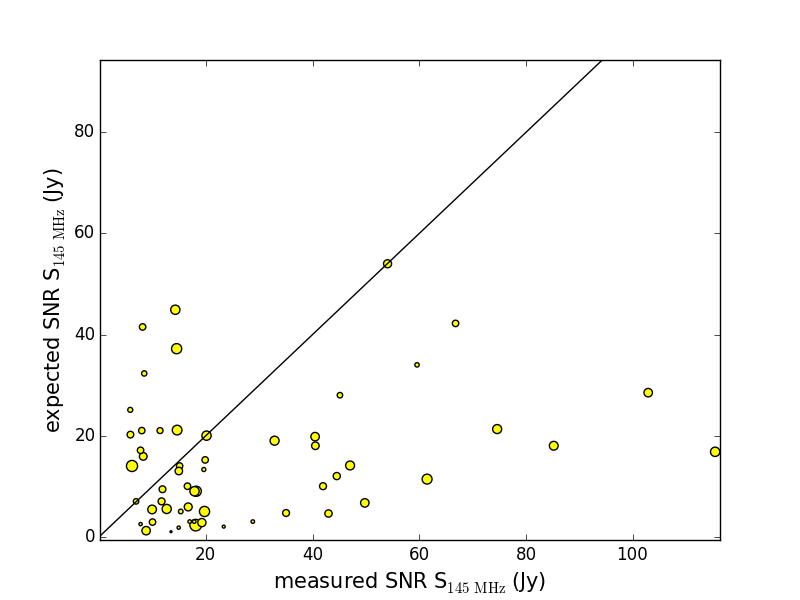
\includegraphics[width=\columnwidth]{figs/PaladiniScatter.png}
\caption{The same comparison as in Figure~\ref{fig:comparisonscatterSNR}, but for the H{\sc{ii}} region fluxes reported by P03 and using a typical spectral index for free-free emission $\alpha=0.1$. All the detected H{\sc{ii}} regions are compact enough to be completely resolved. The size of the point is illustrative of the diameter of the region (as reported by P03, not PAPER), and a black line showing a 1:1 relation is overlaid.}
\label{fig:comparisonscatterHii}
\end{figure}

\begin{table*}
\caption{Measured properties of P03 {H\sc{ii}} regions}
\begin{tabular}{lllcccc}
\hline
ID & R.A. & Dec & SMA$^a$ (P03) & $S_{2.7\,{\rm GHz}}$ & SMA (This work) &  $S_{145\,{\rm MHz}}$	 \\
($l\,b$)   & (deg) & (deg) & (arcmin) & (Jy) & (arcmin) & (Jy) \\
\hline
006.0-01.3	&	271.054	&	-24.4164	&	4	$\pm$	1	&	45	$\pm$	5	&	30	$\pm$	6	&	14	$\pm$	3	\\
006.3+02.0	&	268.101	&	-22.5078	&	4	$\pm$	1	&	1.2	$\pm$	0.7	&	20	$\pm$	4	&	9	$\pm$	3	\\
015.0-00.7	&	275.107	&	-16.2356	&	3	$\pm$	1	&	489	$\pm$	75	&	22	$\pm$	3	&	12	$\pm$	3	\\
017.0+00.9	&	274.625	&	-13.7169	&	5	$\pm$	1	&	21	$\pm$	7	&	24	$\pm$	4	&	15	$\pm$	3	\\
265.2+01.5	&	134.961	&	-43.7636	&	1.2	$\pm$	0.4	&	25	$\pm$	3	&	18	$\pm$	3	&	6	$\pm$	3	\\
267.9-01.1	&	134.685	&	-47.5067	&	1	$\pm$	1	&	153	$\pm$	22	&	26	$\pm$	2	&	167	$\pm$	3	\\
269.2-01.4	&	135.628	&	-48.6822	&	3	$\pm$	1	&	16	$\pm$	2	&	23	$\pm$	5	&	8	$\pm$	3	\\
274.0-01.1	&	141.152	&	-51.9536	&	1	$\pm$	1	&	32	$\pm$	5	&	21	$\pm$	3	&	8	$\pm$	3	\\
281.0-01.5	&	149.796	&	-56.8481	&	2	$\pm$	1	&	9	$\pm$	1	&	24	$\pm$	4	&	12	$\pm$	3	\\
282.2-01.1	&	152.006	&	-57.2406	&	5	$\pm$	3	&	11	$\pm$	2	&	39	$\pm$	5	&	61	$\pm$	3	\\
285.3-00.1	&	157.883	&	-58.0994	&	0.9	$\pm$	0.3	&	13	$\pm$	1	&	28	$\pm$	4	&	20	$\pm$	2	\\
286.2-00.2	&	159.273	&	-58.6372	&	5	$\pm$	2	&	37	$\pm$	4	&	20	$\pm$	2	&	15	$\pm$	3	\\
289.1-00.4	&	164.15	&	-60.1506	&	2	$\pm$	1	&	14	$\pm$	5	&	24	$\pm$	4	&	15	$\pm$	3	\\
293.6-01.3	&	172.184	&	-62.6636	&	5	$\pm$	3	&	5	$\pm$	2	&	31	$\pm$	5	&	20	$\pm$	2	\\
295.0-01.7	&	174.876	&	-63.4583	&		$<$	8	&	12	$\pm$	4	&	27	$\pm$	2	&	45	$\pm$	2	\\
295.2-00.6	&	175.945	&	-62.4517	&		$<$	14	&	20	$\pm$	6	&	21	$\pm$	2	&	20	$\pm$	3	\\
302.5-00.7	&	191.886	&	-63.5686	&	4	$\pm$	2	&	5	$\pm$	1	&	14	$\pm$	2	&	10	$\pm$	4	\\
303.5-00.7	&	194.133	&	-63.5664	&	5	$\pm$	3	&	9	$\pm$	1	&	30	$\pm$	5	&	18	$\pm$	2	\\
305.5+00.0	&	198.474	&	-62.76	&	4	$\pm$	1	&	29	$\pm$	3	&	30	$\pm$	2	&	103	$\pm$	4	\\
305.7+01.6	&	198.598	&	-61.1486	&	3	$\pm$	1	&	6	$\pm$	1	&	29	$\pm$	6	&	17	$\pm$	2	\\
314.0+01.0	&	215.376	&	-59.9225	&		$<$	0.5	&	1.0	$\pm$	0.3	&	18	$\pm$	1	&	13	$\pm$	3	\\
318.0-00.7	&	224.047	&	-59.8714	&		$<$	5	&	7	$\pm$	2	&	13	$\pm$	2	&	7	$\pm$	4	\\
320.7+00.2	&	227.764	&	-57.7736	&	5	$\pm$	2	&	9	$\pm$	3	&	29	$\pm$	5	&	18	$\pm$	2	\\
321.1-00.5	&	229.092	&	-58.1653	&	2	$\pm$	1	&	21	$\pm$	7	&	20	$\pm$	4	&	8	$\pm$	3	\\
322.3-01.2	&	231.721	&	-58.1025	&		$<$	2	&	2	$\pm$	1	&	19	$\pm$	1	&	23	$\pm$	3	\\
326.3+00.7	&	235.583	&	-54.2297	&	6	$\pm$	7	&	14	$\pm$	5	&	11	$\pm$	1	&	6	$\pm$	4	\\
326.6-00.5	&	237.263	&	-54.9933	&		$<$	12	&	18	$\pm$	6	&	32	$\pm$	3	&	85	$\pm$	3	\\
340.1-00.2	&	252.051	&	-45.3003	&		$<$	4	&	5	$\pm$	2	&	25	$\pm$	4	&	15	$\pm$	3	\\
353.6-00.1	&	262.472	&	-34.3953	&	3	$\pm$	1	&	7	$\pm$	2	&	20	$\pm$	2	&	12	$\pm$	3	\\
\hline
\end{tabular}
\\
$^a$ In the cases where the uncertainty in the P03 SMA is greater than the SMA itself, we report a 1$\sigma$ upper limit\\
\label{tab:hii}
\end{table*}

Minimizing $\chi^2(\alpha) = \frac{|S_{\rm measured} - S_{\rm expected}|^2}{\sigma_{\rm measured}^2 + \sigma_{\rm expected}^2}$, where $S_{\rm measured}$ is the PAPER measurement at 145\,MHz,  $S_{\rm expected}=S_{\rm HII}\left(\frac{2.7\,{\rm GHz}}{145\,{\rm MHz}}\right)^{\alpha}$ and $S_{\rm HII}$ is the synthetic 2.7\,GHz flux of the H{\sc ii} region reported by P03, we recover an average favoured value of $\alpha=0.1\pm0.4$.

XXX INTERPRETATION??? XXX

\subsection{Extragalactic sources}

Twenty-eight of the MRC extragalactic point sources detected by the \cite{Jacobs.11} PAPER survey overlapped with our SGP cut and were recovered. A comparison of the fluxes reported in their work with ours allows us to verify our calibration. This comparison is shown in Figure~\ref{fig:exgal}, along with a best-fitting linear relation:

\begin{equation}
S_{145\,\rm{MHz}}^{\rm{Jacobs+`11}} = (0.8\pm0.3) S_{145\,\rm{MHz}}^{\rm{This\,work}} + (8\pm4)
\label{eq:PScal}
\end{equation}

The gradient of the fit is within $1\sigma$ or direct proportionality, and we see a 4--8 Jy offset between our fluxes. However, taking into account the corrections to the \cite{Jacobs.11} flux scale, presented in \cite[][see Section 3 of their paper]{Jacobs.13}, the margin closes to a direct proportionality. 

XXX NEED TO GET EXACT NUMBERS FROM DANNY XXX

\begin{figure}
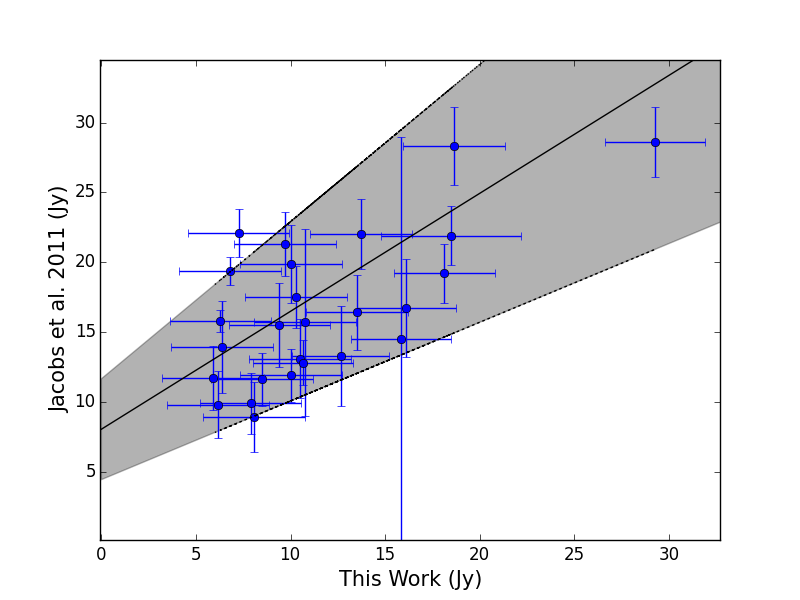
\includegraphics[width=\columnwidth]{figs/Jacobs_Comparison.png}
\caption{A comparison of the fluxes of extragalactic MRC sources measured by \protect\cite{Jacobs.11} at 145\,MHz, compared to our own. The measurements are consistent to within 1$\sigma$. The offset from direct proportionality is accounted for by corrections in \protect\cite[][see Section 3 of their paper]{Jacobs.13}.  A line of best fit is shown (solid line) along with $\pm1\sigma$ on the best fit parameters (shaded region).}
\label{fig:exgal}
\end{figure}

\subsection{Uncatalogued sources}

We detect 23 objects that were isolated enough to confidently measure their flux density, but were not identified as SNRs, {H\sc{ii}} regions, or MRC extragalactic sources.  For these sources, we used the astroquery package for Python to reference the SIMBAD database.  The search radius was set as the angular radius of the object from PAPER with a minimum of 15 arcmin due to the size of the primary PAPER beam.  Astroquery retrurned nearly 3000 objects in total, with the vast majority being stars.  We focused on SIMBAD results of inter-stellar bubbles,  {H\sc{ii}} regions, or radio sources.  

One source identified on PAPER (159) had eight bubble counterparts matched by astroquery, among dozens of stars and various other sources.  Two  sources have {H\sc{ii}} matches; source 146 has one counterpart and source 159 has two, yet neither is convincing as a complete match.  There are fourteen sources that have radio matches (62, 102, 114, 127, 135, 146, 148, 158, 159, 193, 194, 200, 201, 218) with many duplicates.  Source 102 had both a cm radio matcha as well as a radio galaxy match.  The ``Radio(cm)" match might be the one detected by PAPER, since its detects at 21cm wavelengthss.  

\section{Discussion}
\label{sec:disc}


As mentioned in Section~\ref{sec:intro}, the SNR Defect refers to the as yet undetected, yet predicted galactic remnants from calculations based on star formation rates and evolution \citep{Li.91,Pavlovic.13}.  Selection effects are the most likely cause of the ``missing" remnants, as described in \cite{Brogan.06}, which would imply that PAPER should find all the SNRs that are not restricted by the limitations of the survey itself.  We test this with the 294 G14 SNRs.  

In order to analyse the ability of PAPER to detect these SNRs, we remove those PAPER could not reasonably fnd due to its own limitations, which allows for a comparison between the 79 of G14 remnants detected (26.9\%) and the number that we should have found.  

Starting with the range limitation, PAPER covers galactic latitudes $0 < \ell < 40$ \& $200 < \ell < 360 \deg$.  We applied cuts at $24 \deg$ and $232 \deg$ given the nature of PyBDSM to detect image artifacts instead of object candidates beyond these bounds.  The effective range of PAPER ($|b| < 7.5 \deg, 0 < \ell < 24$ \& $232 < \ell < 360 \deg$) contains 189 of G14 SNRs.  With only the range limitation, PyBDSM detected 41.8\% of the remnants.  This limitation is by far the most physically relevant since no remnant outside these bounds has any detections. 

Due to the $5\sigma$ requirement for PyBDSM peak spectral flux detection, objects with a peak flux below $10 Jy$ are highly unlikely to be considered candidates, leading to the second limitation on PAPER.  We scaled Green’s given fluxes at 1GHz to PAPER’s 145 MHz for comparison.  There are 200 of the G14 SNRs with fluxes above $10 Jy$, so PyBDSM detected 39.5\% of these with this limitation.  Combining the flux and range limitations results in 129 of G14 remnants remaining, since there is limited overlap between the two limitation.  In this regime, PyBDSM detects 61.2\%.  

The final limitation is that of object angular size.  PAPER does not resolve objects with a radius greater than $1$ degree, which leaves 251 of G14 SNRs remaining, meaning PyBDSM found 31.5\% of them.  

\begin{table*}
\caption{Summary of PAPER Limitations Applied to Green's SNRs.}
\begin{tabular}{lcccc}
\hline
PAPER Limitation &	Number of G14 SNRs &	Percentage of G14 SNRs & PyBDSM Detection Rate$^*$ & G14 PyBDSM Missed  \\
\hline
Range 					&	189	&	64.3	&	41.8	&	110 	\\
Size 					&	251	&	85.4 &	31.5	&	172		\\
flux 					&	200 &	68.0 	& 	39.5	&	121     \\
Range and Size 			&   181 &   61.6  &   43.6  &   102  	\\
Range and Flux 			&   129 &   43.9  &   61.2  &   50      \\
Size and flux   		&   165 &   56.1  &   47.9  &   86      \\
All Three limitations   &   125 &   42.5  &   63.2  &   46      \\
\hline
\end{tabular}
\label{tab:Defect}
\\
$^*$ 79 detected
\end{table*}

Combining all three limitations yields a total of 125 of the 294 G14 SNRs that PAPER could detect, resulting in a 62.3\% detection rate and 46 remnants that were missed by PyBDSM.  Table~\ref{tab:Defect} below summarizes this analysis.

\section{Conclusions}
\label{sec:conc}

In this work we have presented a low-resolution survey of the SGP at 145\,MHz. Concentrating on SNRs, most of which have not been previously measured at low radio frequencies, we present these novel low-frequency flux densities, as well as possible evidence of synchrotron self-absorption in 31 G14 SNRs. We also measure the flux densities 10 compact G14 SNRs that have complex geometries. Their geometries have limited previous measurements of their flux densities, but PAPER's low-resolution washed out these details, and we were able to provide some of the first high-confidence measurements of the flux densities of these regions.

We additionally  present an analysis of the causes of the phenominon we coined the ``SNR Defect," or the galactic SNRs predicted by star formation rates but undetected observationally.  Looking at the physical limitations of the PAPER survey itself, we found that only 125 G14 sources were physically detectable by PyBDSM, of which we found 79.  This suggests that approximately two-thirds of the SNR Defect can be accounted for by selection effects resulting from the telescope itself.  Other selection effects include the inverse-square law on remnants further away, and superposition of closer remnants interfereing with detection of further ones \citep{Brogan.06}.  Our results suggest that most if not all of the SNR Defect is due to selection effects and not faulty predictions.  

We also have evidence for what appears to be a lack of spectral turnover in 29 {H\sc{ii}} regions, suggesting a previously unaccounted-for component of free-free emission for these objects.

XXX {\bf any discussion of exgal sources?}

As for the 23 unclassified objects, we found that most of these match real objects; however, the detections provided by PAPER alone are not enough to determine which of the SIMBAD candidates we found.  Since none of the sources matched any SNRs and only one matched {H\sc{ii}} regions, it is unlikely that our numbers would change considerably regardless of the quality of matches.  

Approximately 40\% of our detections could not be confidently analysed due to the high amount of confusion in the most crowded regions of the SGP, given PAPER's low resolution. Upcoming low-frequency surveys such as GLEAM will have the resolution and precision to constrain the nature of these objects.

The data presented here was correlated using only one of the two instrumental polarizations PAPER is capable of measuring. Dual-polarization measurements, and the intrinsic polarization of SNRs \citep[e.g.][]{Gao_v.11} should allow the steadfast confirmation of the nature of these regions in the SGP. Work on these measurements is currently in progress, and will be presented in a future study. Meanwhile, the HERA\footnote{\url{www.reionization.org}} instrument is currently under construction at the PAPER site in South Africa. This instrument will have far superior sensitivity ($\sim\times40$ per antenna) and resolution at low-frequencies (50--250\,MHz), and the authors look forward to presenting sky survey data with it.

\section*{Acknowledgements}
This work made use of the TOPCAT package\footnote{\url{http://www.star.bristol.ac.uk/~mbt/topcat/}} and the SIMBAD database, operated at CDS, Strasbourg, France.
We thank SKA-SA for their efforts in ensuring the smooth running of PAPER. PAPER is supported through the NSF-AST program (awards 0804508, 1129258, and 1125558), the Mt. Cuba Astronomical Association, and by significant efforts by staff at NRAO. 

\bibliographystyle{plainnat}
\bibliography{snrbib_MNRAS_version}{}

\end{document}
